\documentclass[11pt,a4paper]{article}

\usepackage[margin=2.5cm]{geometry}
\usepackage{graphicx}
\usepackage{amsmath}
\usepackage{hyperref}
\usepackage{booktabs}
\usepackage{enumitem}
\usepackage{titlesec}
\usepackage{caption}
\usepackage{subcaption}
\usepackage{float}
\usepackage{natbib}
\usepackage{listings}

\titleformat{\section}{\large\bfseries}{\thesection}{1em}{}
\titleformat{\subsection}{\normalsize\bfseries}{\thesubsection}{1em}{}

\title{Computación de Altas Prestaciones (CAP)\\
Trabajo prácticas de laboratorio sesión 1 }

\author{
Estudiante: Juan Camilo España Lopera\\
Profesor: Dario Gonazales Lema\\\\
Universidad de Oviedo
}

\date{\today}

\begin{document}

\maketitle

% -------------------------------------------------
\section{Error en estimación de tiempos}

Para cuantificar la variabilidad inherente a las mediciones de tiempo, se ejecutó una misma configuración en 30 ocasiones (columnas = filas = 1536, tamaño de bloque = 512, repeticiones = 30) y se calculó la desviación estándar para cada estrategia (Tabla~\ref{fig:error_est}). Los resultados presentan porcentajes de desviación respecto a la media
entre el 1\,\% y el 1.5\,\%, lo que permite establecer que diferencias de tiempo
inferiores a ese margen no deben considerarse significativas, mientras que diferencias
superiores podrían reflejar un efecto real del parámetro evaluado

\begin{figure}[ht]
    \centering
    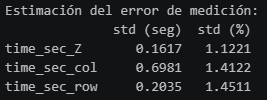
\includegraphics[width=0.4\textwidth]{images/error_estimaciones_tiempo.png}
    \caption{Estimación de error de tiempos de ejecución en 30 corridas}
    \label{fig:error_est}
\end{figure}



\section{Estimación del tamaño de bloque}

Antes de variar el tamaño de las matrices, se determinó primero el tamaño de bloque $b$ para la multiplicación por bloques, ya que este parámetro solo afecta a esa estrategia. Para esta experimentación solo se corrió la multiplicación de z order y se comentaron las otras dos. Fijado el valor óptimo, se estudió luego cómo cambia el tiempo de cómputo al modificar el tamaño de las matrices.

El algoritmo por bloques divide las matrices en submatrices de $b \times b$ para reutilizar datos en caché antes de su desalojo. Se busca que los tres bloques activos a la vez (uno de $A$, uno de $B$ y uno de $C$) quepan simultáneamente en caché (dada la forma en que se multiplican las matrices elemento a elemento no todos los bloques deberían caber en caché pero se hizo este supuesto para tener una estimación inicial de valores de bloques). Con \texttt{int} de 4 bytes, la restricción es
\[
3 b^2 \cdot 4 \leq C_{\text{size}} \quad\text{y}\quad b \leq \sqrt{\frac{C_{\text{size}}}{12}}.
\]

Con las características del nodo CPU del clúster (Figura~\ref{fig:cache_cpu_hpc}), para L1 se tiene $C_{\text{size}} = 48$ KiB y para L2, $C_{\text{size}} = 418$ KiB, por lo que los límites son $b \approx 64$ (L1) y $b \approx 418$ (L2).

Además, cada línea de caché tiene 64~bytes, es decir, almacena
$64/4 = 16$ enteros contiguos. Para evitar que un bloque empiece o termine en medio de
una línea de caché, se eligieron valores de $b$ múltiplos de 16.
\begin{figure}[ht]
    \centering
    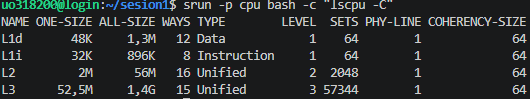
\includegraphics[width=0.8\textwidth]{images/cache_CPU_HPC.png}
    \caption{Características de la caché del nodo CPU del clúster HPC.}
    \label{fig:cache_cpu_hpc}
\end{figure}

Asimismo, se exige que $b$ divida exactamente la dimensión $n$ de la matriz
($n \bmod b = 0$), para eliminar la sobrecarga de comprobar si un bloque excede los
bordes. Esto simplifica el código y produce mediciones más limpias. Por ello, tanto los
valores de $b$ como los de $n$ se fijaron como múltiplos de todos los bloques, además se inició en un valor bajo de b se finalizó en uno alto para ver la evolución. A continuación los valores utilizados que se encuentran programados en la primera parte del archivo experimentos.py:
%
\[
b \in \{8,\;16,\;32,\;64,\;128,\;256,\;512\;1024\},
\qquad
n \in \{1024,\;2048,\;3072\}
\]
%

Como resultado de la experimentación se obtuvieron los datos mostrados en las Figuras \ref{fig:z_experiments} y \ref{fig:diff_bloq}. El mejor rendimiento se alcanzó utilizando un tamaño de bloque de 512 para las matrices de 1024 y 2048, mientras que, para la matriz de 3072, el desempeño óptimo se logró con bloques de 1024, sin embargo, las diferencias para bloques (256, 512 y 1024) no superan el margen de error identificado en la sección anterior. Para continuar con los análisis, se empleará un tamaño de bloque de \textbf{$b=512$}.

\begin{figure}[h]
    \centering
    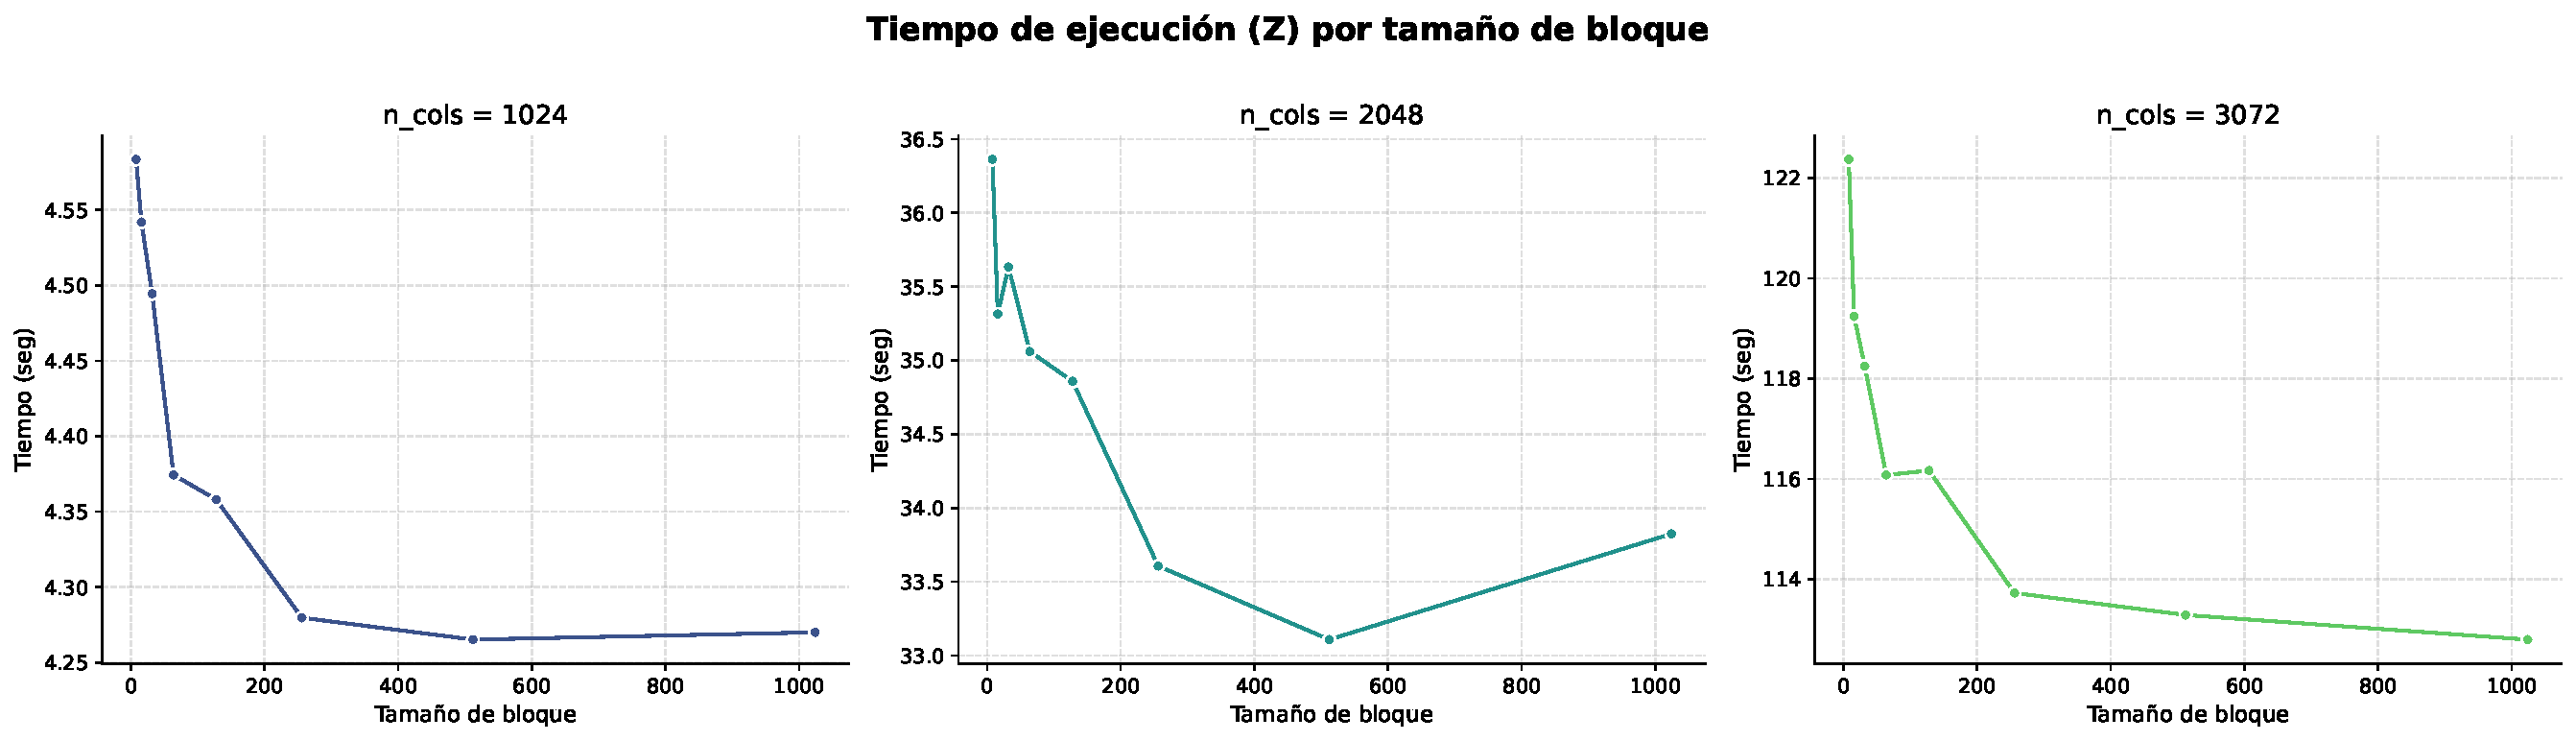
\includegraphics[width=0.8\textwidth]{images/block_experiments_Z.pdf}
    \caption{Tiempo de ejecución vs tamaño de bloque y dimensions matrices}
    \label{fig:z_experiments}
\end{figure}

\begin{figure}[h]
    \centering
    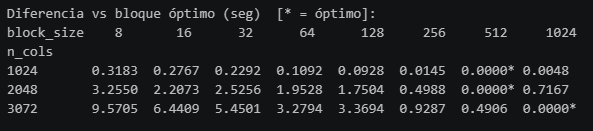
\includegraphics[width=0.6\textwidth]{images/diff_tam_bloq.png}
    \caption{Diferencias en tiempo vs bloque óptimo}
    \label{fig:diff_bloq}
\end{figure}



\newpage


\section{Comparación de tiempos entre métodos de acceso}

Los resultados muestran que el acceso por columnas (\textit{column-major}) es consistentemente el método más lento, y esta diferencia se acentúa con el tamaño de la matriz: mientras que para 1024×1024 la diferencia frente a \textit{row-major} es de apenas 7 segundos, para 5120×5120 supera los 2160 segundos. Esto se explica por los fallos de caché que genera el acceso no contiguo a memoria en matrices almacenadas en orden de fila, penalización que crece cuadráticamente con el tamaño.

Entre \textit{row-major} y \textit{Z-order}, los tiempos son muy similares para matrices pequeñas, dentro del margen de error, pero \textit{row-major} toma ventaja en matrices grandes. Esto se debe a que la implementación de \textit{Z-order} introduce un sobrecosto en los índices de los bloques externos: con bloque fijo de 512, a mayor tamaño de matriz más iteraciones recorren los loops de bloques, acumulando sobrecosto. Adicionalmente, la asignación de memoria con \texttt{malloc} sigue el esquema contiguo por filas, lo que favorece naturalmente a \textit{row-major}. Si la memoria se asignara en bloques contiguos alineados con el patrón Z, el método podría aprovechar mejor la localidad de caché y recuperar competitividad frente a \textit{row-major}.

Esto también podría explicar por qué un tamaño de bloque mayor obtuvo mejores resultados en el análisis, ya que empieza a reducir los costos de índices y se comporta de forma más similar a un esquema row major.

\begin{figure}[h]
    \centering
    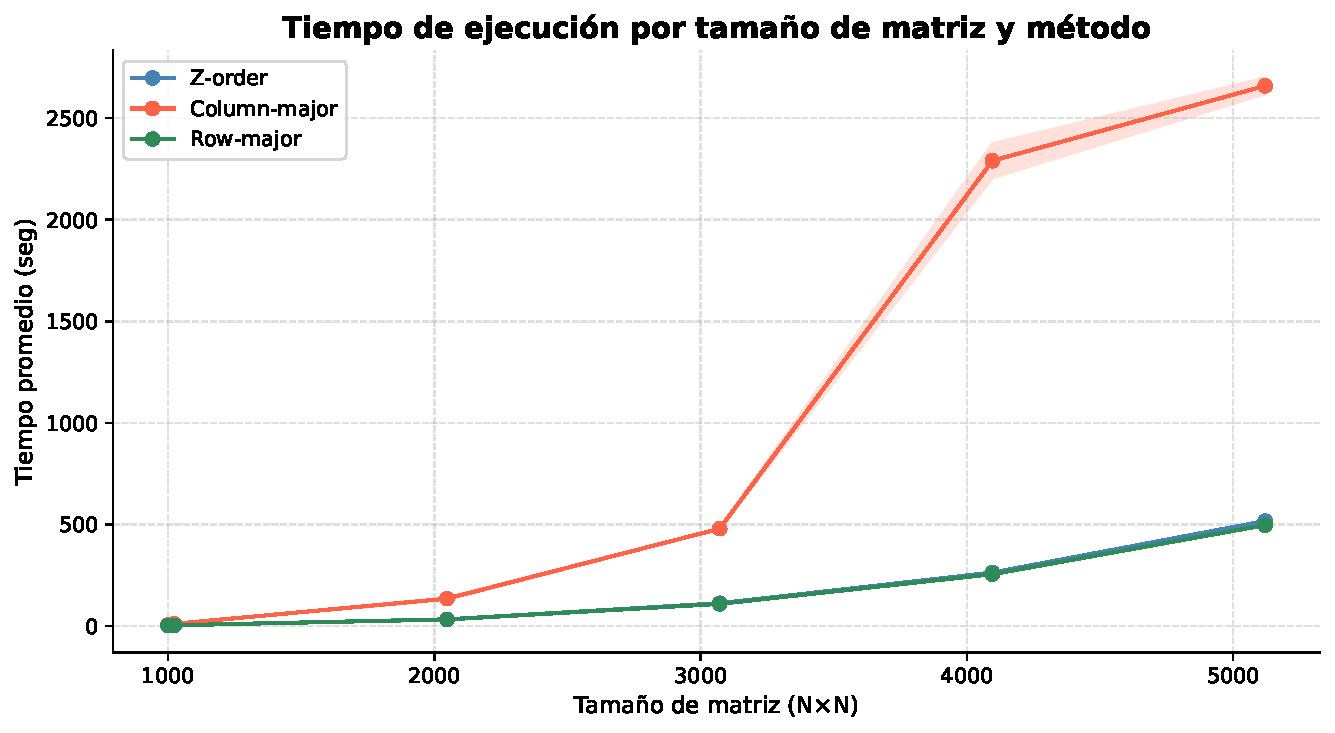
\includegraphics[width=0.5\textwidth]{images/matrix_size_comparison.pdf}
    \caption{Comparación de los métodos en función de las dimensiones de las matrices}
    \label{fig:comparison_metodos_tamanos}
\end{figure}





\begin{figure}[h]
    \centering
    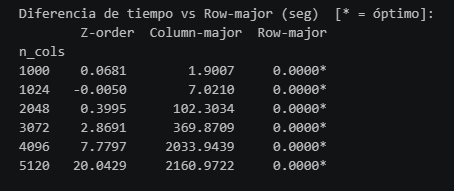
\includegraphics[width=0.5\textwidth]{images/comp_metod_matsize.png}
    \caption{Differencias de métodos vs Row Major}
    \label{fig:tab_met_size}
\end{figure}




\section{Dificultades y otros Análisis}

\subsection{Asignación de espacios de memoria RAM}
Un aspecto previo a resolver fue la forma de asignar memoria en RAM para las matrices,
ya que el método de asignación puede afectar el rendimiento por su impacto en la
contigüidad de los datos. Se evaluaron dos alternativas: la primera reserva cada fila
de forma independiente con \texttt{malloc}, lo que puede ubicar filas en zonas dispersas
de memoria y desaprovechar la localidad espacial; la segunda reserva un único bloque
contiguo para toda la matriz y asigna a cada puntero de fila su posición dentro de ese
bloque. El segundo método produjo tiempos consistentemente menores, por lo que se adoptó
como asignación por defecto. Ambas implementaciones se muestran a continuación, con la
primera comentada a modo de referencia.


\begin{lstlisting}[language=C]
Metodo 1: filas independientes (descartado)
// int **matrix = malloc(rows * sizeof(int *));
// for (int i = 0; i < rows; i++)
//     matrix[i] = malloc(columns * sizeof(int));
 
 Metodo 2: bloque contiguo (adoptado)
int **matrix = malloc(rows * sizeof(int *));
int *block   = malloc(rows * columns * sizeof(int));
for (int i = 0; i < rows; i++)
    matrix[i] = block + i * columns;
\end{lstlisting}

En cuanto a la asignación de los espacios de memoria, se empleó un esquema row-major, el cual coincidía con el algoritmo de acceso del mismo tipo para la maultiplicación, favoreciendo así el desemepeño de esta. La disposición en memoria de las matrices debe corresponder al patrón de acceso que se utilizará posteriormente para aprovechar al máximo la eficiencia, tal como se menciona en el trabajo de \citet{chatterjee1999recursive}.

\subsection{Guardas de límite en la multiplicación por bloques (Z-order)}

Durante la experimentación los guardas de límite (\texttt{\&\& i < rows}, \texttt{\&\& k < rows}, \texttt{\&\& j < columns}) en los loops internos de \texttt{zorder\_mul} fueron eliminados deliberadamente, ya que introducen una comparación adicional en el loop más interno, lo que aumenta de forma significativa la cantidad de operaciones realizadas y afecta la medición del rendimiento puro del acceso a memoria por bloques. Para garantizar resultados válidos, todos los experimentos usaron combinaciones donde \texttt{block\_size} divide exactamente la dimensión de la matriz. En la versión entregada los guardas fueron restituidos para prevenir accesos fuera de los límites del arreglo en caso de que se utilicen parámetros arbitrarios, evitando comportamiento indefinido o segmentation faults.

\subsection{Gestión de archivos de salida}

En los primeros experimentos los archivos de salida se nombraban con timestamp, lo cual no presentó inconvenientes. Sin embargo, en el último experimento, al lanzar múltiples jobs en paralelo con mayor frecuencia, se detectó que varios jobs obtenían el mismo timestamp, causando colisiones y pérdida de resultados. Por esta razón, en ese experimento se modificó el script de lanzamiento para nombrar los archivos usando el job ID asignado por SLURM (\texttt{\%j}), garantizando unicidad sin depender del tiempo de lanzamiento. Este último formato de nombramiento es que se dejo en la entrega del código.



\bibliographystyle{plainnat} 
\bibliography{ref}

\end{document}